%************************************************
\chapter{Introduction}
\label{ch:introduction} %
%************************************************

{\sffamily\slshape This chapter is based on the text from Section 1 of the published versions of the preprints at \href{https://arxiv.org/abs/2411.15900}{arXiv:2411.15900} and \href{https://arxiv.org/abs/2504.10609}{arXiv:2504.10609}.\\}

Networks of molecules interlinked by chemical reactions are recurrent in real-world scenarios: cellular metabolic processes, interactions among atmospheric constituents, environmental phenomena such as cycling of nutrients and pollutants, the human gut microbiome, and industrial chemical reactors.
This is because in practical scenarios, reactions are rarely encountered in isolation. Rather, they are components of larger interconnected networks, where the products of one reaction may be the reactants of numerous other reactions. Such networks are called \emph{reaction networks}.
Modeling these networks is challenging due to the inherent complexities of such systems.
One type of complexity arises from nonlinear dynamics, which appear in particular when transcending one-to-one reactions.
Another type of complexity arises from the existence of parallel and alternative sequences of reactions,
termed pathways, which may give the same overall effect but involve distinct yet intersecting sets of molecules.
Such pathways in reaction networks are manifested in diverse contexts:
metabolic pathways in organisms for cellular metabolic networks, nutrient cycles in the environment, and synthesis plans in chemical reaction networks.

\begin{figure}[!t]
    \centering
    \begin{subfigure}{0.48\textwidth}
        \centering
        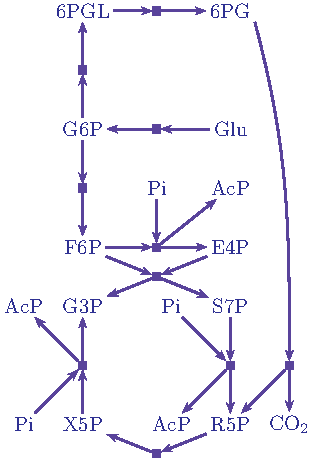
\includegraphics[width=\textwidth]{graphics/prolog/crn_metabolite.pdf}
        \caption{a reaction network showing the metabolism of carbohydrates~\cite{crn_metabolite}}
        \label{fig: crn1}
    \end{subfigure}%
    \hfill
    \begin{subfigure}{0.48\textwidth}
        \centering
        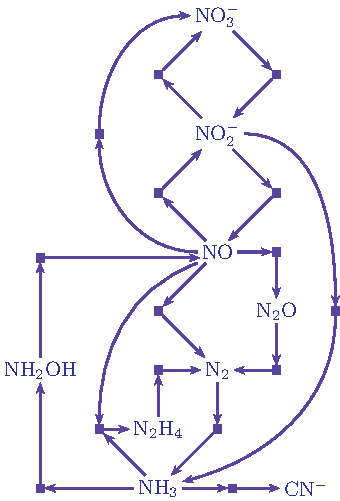
\includegraphics[width=\textwidth]{graphics/prolog/crn_atmosphere.pdf}
        \caption{a reaction network showing the reactions of atmospheric nitrogen~\cite{crn_atmosphere}}
        \label{fig: crn2}
    \end{subfigure}
    \vspace{0.5cm}
    \\
    \begin{subfigure}{\textwidth}
        \centering
        \vspace{0.5cm}
        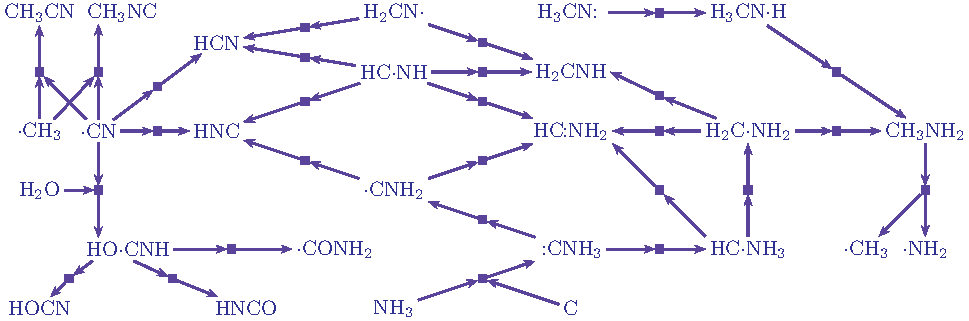
\includegraphics[width=\textwidth]{graphics/prolog/crn_astronomy.pdf}
        \caption{a reaction network showing reactions in the interstellar medium~\cite{crn_astronomy}}
        \label{fig: crn3}
    \end{subfigure}
    \vspace{0.2cm}
    \caption{Three chemical reaction networks from diverse contexts, attempting to show that reaction networks can be used to model diverse environments.}
    \label{fig: crns}
\end{figure}


The exploration of reaction networks to synthesize molecules has primarily been done experimentally in the wet laboratory. However, this process is labor intensive, costly, and limits the pace of exploration. \emph{In silico} modeling and exploration of reaction networks have the potential to speed up the process and guide manual efforts. The finer the physical details included in the modeling of the reaction networks, the more accurate the results can be expected to be. The ultimate way of doing that would be to construct the complex free energy landscape for the full reaction network, which then, in principle, would allow for the full simulation of reactions, as these are ultimately guided by the laws of thermodynamics.
However, this might be currently past any modeling and computational capacities available. 
Presently, algorithmic exploration of reaction networks by automated tools such as Reaction Mechanism Generator (RMG)~\cite{rmg2}, Chemotron~\cite{chemotron}, Yet Another Reaction Program (YARP)~\cite{yarp} and others, is limited to predicting a short sequence of reactions to a queried target molecule (often with no possible side-products). These tools have been applied to domains such as combustion chemistry~\cite{rmg2}, synthesis planning~\cite{retrosynthesis_comp,retrosynthesis_comp2,retrosynthesis_comp2}, reactions in metabolic systems~\cite{metabolic_comp,metabolic_comp2}, batteries, the atmosphere, the interstellar medium and so on. 
The diversity and varying approaches taken in characterizing reaction networks is evidence to the fact that generic methods are absent which work reasonable well across multiple and vastly differing application scenarios.

\section{Thermodynamics and Reaction Networks}

Equilibrium thermodynamics has been often used to determine the spontaneity of an isolated chemical reaction. Specifically, from the Gibbs free energy one can find the driving forces behind a reaction and determine whether its occurrence is favorable or not. Specifically in the context on reaction networks, chemical potentials can be used to determine if a given reaction is favorable in thermodynamical terms, and then only the favorable reactions are used in the exploration of the reaction networks.

However, before one can search for pathways in a reaction network, the network itself has to be constructed. This can be done in various ways. In one approach, the potential energy surface of a set of molecules is explored to elucidate trajectories with low-lying saddle points, separating the reactants from the products. Computationally intensive quantum mechanical calculations are used in most cases \cite{crn_expand_qm,crn_expand_qm3}, along with faster but less accurate semi-empirical methods in some \cite{yaks,empi1}.
Recently, generative diffusion models have also been used to perturb molecules to generate reaction networks with unknown mechanisms \cite{OA-ReactDiff,diffusion_ai}.
A different approach is to use reaction templates for iteratively expanding the network from a set of starting molecules, possibly in conjunction with filters to exclude specific reactions \cite{rmg2,molpher}.
Further approaches include the generation of the reaction network of interest in a one-shot heuristical process by an expert \cite{heuristic_expert}, or the loading of an existing network from a database \cite{reported_network}.

Once a reaction network is constructed, pathways can then be queried in the network using diverse strategies. Some general methods to search and analyze pathways in reaction networks can be found at \cite{search_crn} and ~\cite{search_crn2}. Previous work include Beam search based on suitable crafted scoring functions utilizing priority queues \cite{beam_search_pq}, as well as Monte-Carlo search trees extended with a method to sample efficient pathways \cite{mc_trees}.
Traditional path-finding algorithms such as A$^*$ algorithm~\cite{shortest_path_hypergraph2} and cutting-plan algorithm for an integer linear program~\cite{shortest_path_hypergraph1} have been used in previous work to find pathways between molecules.
Some analytical strategies have been used in the study of dynamics of pathways in reaction networks \cite{crn_dynamics,crn_dynamics2}, but they are often limited by the availability of kinetic data and the scale of the networks.

Moving on to studies specifically using thermodynamics to elucidate pathways in reaction networks, an example would be of~\cite{synthesis_planning_CRN_thermodynamics} which uses data provided by thermochemistry to suggest pathways in reaction networks through pathfinding algorithms and a linear combination of the lowest cost pathways in that network. 
In thermodynamics-based metabolic flux analysis~\cite{hatz_thermo_flow}, the mass balance constraints of metabolic flux analysis are augmented by additional thermodynamic constraints to produce flux distributions and metabolite activity profiles free from thermodynamic infeasibilities.
In \cite{seifert_thermodynamics_CRN_JCP}, nonequilibrium thermodynamics was developed to explore reaction networks, employing a stochastic trajectory-based approach to define energy, entropy, and heat dissipation along reactions.
Building upon stochastic thermodynamics, a nonequilibrium thermodynamic framework for open reaction networks has been formulated~\cite{esposito_thermodynamics_CRN_PRX}, governed by deterministic rate equations with mass action kinetics and introducing a nonequilibrium Gibbs free energy quantifying the minimal work required to induce nonequilibrium states from an equilibrium state.
This nonequilibrium Gibbs free energy is minimized as the open detailed-balanced network relaxes to an equilibrium state, aligning with the maximum entropy principle.
Circuit theory has been applied to reaction networks~\cite{esposito_circuit_theory_CRN_PRX} extending the chemical analogs of Kirchhoff’s laws to predict reaction currents within complex reaction networks.
\cite{ILP_paper2} utilizes linear programming to identify complex balanced realizations of mass action kinetics in reaction networks.
\cite{ILP_paper2, ILP_paper3, ILP_paper4} have introduced numerical procedures for determining weakly reversible reaction networks using integer linear programming (ILP), emphasizing the importance of ILPs in identifying specific network properties.
Mixed integer linear programming has been employed to prune reaction networks using experimental data and to understand complex chemical systems in~\cite{ilp_CRN_infer}.

Much of the work cited in the preceding paragraph primarily focuses on theoretical formulations, with few executable implementations.
In contrast, MØD~\cite{mod_web,jakob_software} is a software package developed to generate and analyze reaction networks.
M{\O}D models molecules using undirected graphs with attributes, hence with each atom explicitly represented, and reactions are modeled by rules for transforming molecule graphs.
Reaction networks can automatically be generated from a set of rules and a set of starting molecules using the graph transformation engine of M{\O}D.
The outcome is a directed multihypergraph representing the reaction network.
The pathways in such reaction networks can then be queried using integer hyperflows as a formal model~\cite{jakob_integer_hyperflows}
and the reaction network can be queried using computational means for the presence of the specified pathway.
This framework allows for a flexible, yet precise specification of pathways and a search for such pathways by computational means.
However, the methodology~\cite{jakob_integer_hyperflows} currently does not incorporate any dynamics in the modeling of the reaction network.

A critical assumption while using thermodynamics to search for pathways in reaction networks is that the reactions in the network are in equilibrium, and the concentration of the molecules are steady. Given enough time, a reaction network will reach a steady-state where the favourable pathways are determined by the overall free energy landscape, and corresponds to a configuration which has the minimum free energy of the molecules. However, these assumptions might (over)simplify practicalities that might hinder thermodynamically favorable reactions from occurring.

\section{Energy Barriers and Reaction Networks}

Kinetic studies of individual reactions have provided valuable insight into their mechanisms which are often not provided by thermodynamics alone, which in turn can generate ways to optimize the reaction to suit the overall synthesis goals.
Despite the `dynamics' in the name, thermodynamics does not help to elucidate the `dynamics' of the system: how fast does the pathway in question run and how quickly does the system equilibrate? For example, under atmospheric conditions, the conversion of diamond to graphite is thermodynamically favorable. However, the energy barrier for this conversion is high, so, thankfully, for all practical purposes `diamonds are forever'. 
Therefore, kinetic parameters of reactions, such as the free energy barrier or the rate constant, might provide better alternatives for characterizing pathways. Theoretical and computational modeling attempts to offer a possibility for analyzing the kinetics in reaction networks to various degrees of accuracy and computational efficiency, depending on the level of abstraction employed.

Except for approaches where the reaction network is generated by the exploration of the potential energy surface, individual reactions will need to be annotated with the kinetic parameters from a separate source, such as databases \cite{database_energy_barriers}, estimations informed by experiments \cite{reported_network}, or dedicated quantum mechanical calculations \cite{CRN_qm}.
Empirical relations, deduced via machine learning on available data on kinetics of reactions, have been used to estimate kinetic parameters for reactions \cite{ml_energy_barrier,ml_energy_barrier2,ml_energy_barrier3,ml_energy_barrier4,ml_energy_barrier5,ml_energy_barrier6,ml_reaction_barrier7}. However, these methods have limited success on `out of class' molecules \cite{scaling_limitations}. 

Although more expensive, strategies that base the search for pathways in reaction networks based on the kinetics ultimately increase the utility of the search process of pathways to the queried target molecule, with the trade-off of increased computational costs. This is because additional calculations are required to estimate the energy barriers of the reactions (than just computing the chemical potentials of the molecules in the reaction network) but it increases the realism in the resulting search. This results in an approach more faithful in modeling the physical system and which might be of more utility for potential users.

An ideal pathway enumeration algorithm would only explore a subset of reactions in the possible molecular space that are only necessary for the more realistic pathways. One way of quantifying how `realistic' a pathway is (or in other words, how probable it is for the pathway to be observed in a real reactor system) would be to score it using some metric, based on physical parameters. However, it is not generally easy to annotate each reaction with this metric and determine which reaction channels are more favoured in practice. This leads to characterization of more reactions than the minimum required. Many methods use the exploration strategy of characterizing all immediate reaction channels and prioritizing only the ones that are immediately important, for further elucidation of the pathway. This variant of a greedy algorithm considers only the most favoured channel at each steps and ignores the rest completely. A more inclusive and forward-looking algorithm would investigate multiple reaction channels at each step to determine most of the pathways with large contributions to the flow of matter in an attempt to identify the most optimal pathways. However, in reality, unlike in enumerated fixed pathways, the constituent intermediate molecules are not constrained to react only through the reaction specified by the pathway. They reaction through various side reactions resulting in reduction of performance of the pathway than the optimal calculated.

\section{Contribution of this work}

In this work, thermodynamic principles are incorporated into the existing hyperflow model in M{\O}D in Chapter~\ref{ch:thermodynamic_model}.
In particular, we develop methods based on mixed integer linear programming (MILP) that allow thermodynamic constraints to be added to the specification of pathways extending the available search for the pathways in the M{\O}D framework.
Our methods can return several alternative pathways, and these can be ranked on the basis of thermodynamic-based metrics. 
It would be helpful to the reader to point out that in this work, reaction networks are modeled on a level of abstraction where the network is represented by a hypergraph and individual reactions are represented by directed hyperedges \cite{jakob_integer_hyperflows}.
This enables us to capture the many-to-many mapping in chemical reactions which is not possible easily usinging simple directed graphs (with edges directed from one vertex to another vertex).
The nodes of the hypergraph are molecular graphs (with their nodes representing atoms and edges representing bonds) and hence the modeling is atomistically explicit.

We note that returning multiple pathways can significantly increase the practical value of the investigations.
Models of reaction networks and estimations of thermodynamic parameters are inherent simplifications of reality.
Hence, any single pathway returned may turn out to be less desirable in the face of further details of the chemical situation.
Hence, having a number of highly ranked pathways available from which the practitioner can choose is a more robust strategy.

The assignment of chemical potentials to the molecules in the reaction network to calculate the Gibbs free energies for its reactions is done using the semi-empirical method GFN2-xTB~\cite{grimme_xtb} in the current implementation, which provides a good balance between accuracy of the thermodynamic parameters and the ability to handle larger molecules.
However, it can be replaced by any other method to assign chemical potentials if the user desires so.
For generality we refer to the chosen method as a thermodynamic oracle.
We note that using a thermodynamic oracle to calculate the chemical potentials of the molecules in an automated fashion has the added benefit of being applicable in rule-based generative systems where the chemical space is expanded on the fly and the molecules generated are unknown at the start.

To the best of our knowledge, there currently does not exist a computational method for searching for pathways in reaction networks based on thermodynamic constraints that combines MILP with the wide applicability and speed of semiempirical tight-binding methods.

In Chapter~\ref{ch:refined_model}, we further extend the framework developed to incorporate an objective measure to rank pathways in a reaction network maximizing the probability of the entire pathway based on physical principles. 
Based on the notion that energy barriers of reactions are the determining factor for the kinetics of the network, we develop an automated methodology for computing such energy barriers, building on a combination of an array of existing computational tools. A key novelty is that in contrast to the standard manual intervention required to generate reaction trajectories from which the reaction barrier can be estimated, we try to automate this part of the process.
Lastly, we formulate an integer linear program which allows the user to specify queries for pathways in the network in a very flexible and generic way. Solving this integer linear program returns all pathways fulfilling the criteria, ranked by the objective measure mentioned above.
In short, this gives an automated, general, and flexible methodology for analyzing reaction networks, a methodology which offers a speed-up over manual search for pathways but with comparable quality.

To exemplify its utility in Chapter~\ref{ch:casestudy2}, we apply it to a reaction network expanded from the molecules 2-hydroxyethanenitrile, ammonia and water, where we query for pathways to glycine, an amino acid, and 2-hydroxyethanoic acid, a molecule encountered in photorespiration in plants.

\section{Contributing Papers and Overview}

Most of the text and illustrations in this document is taken from the following papers:

\begin{enumerate}
	\item \textsf{\textsl{Pal, Adittya, Rolf Fagerberg, Jakob Lykke Andersen, Christoph Flamm, Peter Dittrich, and Daniel Merkle. "Finding thermodynamically favorable pathways in chemical reaction networks using flows in hypergraphs and mixed-integer linear programming." Journal of Chemical Information and Modeling 65, no. 13 (2025): 6772-6787}}
	
	Chapters 2, 4 and 5 are taken from this peer-reviewed paper, while parts of Chapters 1 and 8 are based on the text from it. 
	
	\item \textsf{\textsl{Pal, Adittya, Rolf Fagerberg, Jakob Lykke Andersen, Peter Dittrich, and Daniel Merkle. "Finding Pathways in Reaction Networks Guided by Energy Barriers Using Integer Linear Programing." Molecular Informatics 45, no. 3 (2026): e70021}}
	
	Chapters 3, 6 and 7 are taken from this peer-reviewed paper, while parts of Chapters 1 and 8 are based on the text from it. 
\end{enumerate}

The rest of this thesis is organized as follows:
In Chapter~\ref{ch:toolbox}, we give the definitions underlying our modeling of reaction networks and pathways.
In Chapter~\ref{ch:preliminaries}, we give an overview of the network construction process by the recursive application of graph transformation rules to an input set of molecular graphs.
In Chapter~\ref{ch:thermodynamic_model}, which constitutes the core part of the work extending the integer hyperflows with thermodynamic constraints and an objective function, we give the details of the proposed framework and comparison with some existing frameworks.
In Chapter~\ref{ch:casestudy1}, we demonstrate the usability of the method proposed in Chapter~\ref{ch:thermodynamic_model} by applying them on a reaction network constructed from hydrogen cyanide, ammonia and water.
In Chapter~\ref{ch:refined_model}, we refine the framework proposed in Chapter~\ref{ch:thermodynamic_model} with energy barriers, an alternative objective function, enumeration of pathways and partial ordering of the molecules in the returned pathways.
In Chapter~\ref{ch:casestudy2}, we demonstrate the usability of the method proposed in Chapter~\ref{ch:refined_model} by applying them on a reaction network constructed from glycolonitrile, ammonia and water.
In Chapter~\ref{ch:conclusion}, we offer a conclusion to the work presented here.
Some additional work have been placed in appendices.

